\emph{Narratology}, or narrative theory, is a literary science that has experienced considerable development over the last hundred years. The topic of narrative theory has been explored by literary theorists across Europe throughout the twentieth century. Consequently, many different typologies and proposals have emerged on how to view the topic of narrative and narrative mode and how to conduct narrative analysis. \cite{kubicek-vypravec}

In this chapter, I introduce some basic narratological concepts. Next, I show a selected typology to demonstrate its relevance to this thesis and focus on the application of narrative theory to creative writing.

\section{Forms of Narrative by Person}
\label{forms-of-narrative}

\emph{Person} is a linguistic category of verbs, based on which the primary forms of narrative are distinguished. In addition to verbs, this form is also manifested in personal and possessive pronouns and some particular conjunctions. In other words, it is a mode of expression that answers the question of \emph{how} to write the story, grammatically speaking.\cite{docekalova}

\paragraph{First-person narrative} is a mode of literary narrative in which the narrator tells the story in the first-person singular. Traditionally, first-person narrative reduces the narrator's omniscience to the subjective perspective, often given by the main character. \cite{vlasin-slovnik}

Nevertheless, there are several modes of first-person narration. These modes differ in the level of subjectivity. \cite{dolezel-narativni-zpusoby}

\paragraph{Third-person narrative} is a mode that is realized in the third person singular. Unlike the first-person narrative, the narrator is traditionally in the role of an objective observer. However, in modern literature, different levels of objectivity can be encountered. Therefore, the differences between the semantic aspects of first and third-person narratives are suppressed. Consequently, the main distinction depends on the syntactic structures of these forms. \cite{vlasin-slovnik}

\paragraph{Other modes of narrative} also exist. There is the \emph{second-person narrative}, which is a less frequent narrative mode. There are also narratives given in plural, but these methods are rarely used.

\section{System of Narrative Modes}

From a number of narrative typologies, I decided to choose the system proposed by Czech linguist and literary theorist Lubomír Doležel. Doležel's system of narrative modes is captured in the tree diagram in Figure \ref{fig:schema-dolezel}.\cite{dolezel-narativni-zpusoby}

\begin{figure}[ht]
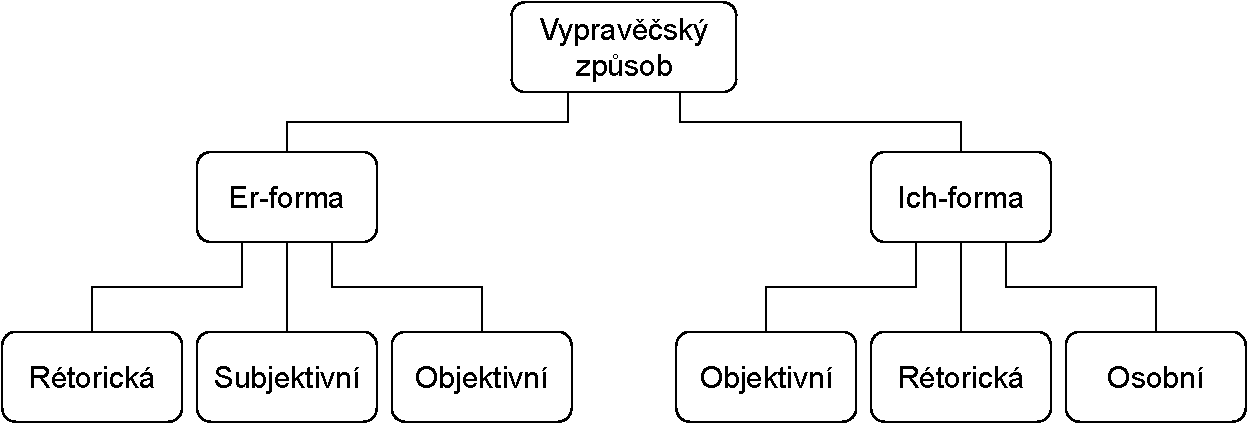
\includegraphics[width=1\textwidth]{data/dolezel-schema.pdf}
\caption{System of narrative modes by Doležel}
\label{fig:schema-dolezel}
\end{figure}

In the section \ref{forms-of-narrative}, I mention some degrees of subjectivity and objectivity of the narrator. The typology offered by Lubomír Doležel is built on the degree of subjectivity and the narrative's person. Similar classifications can be found in various creative writing methodologies \cite{docekalova} since the typology is graspable and intuitive for writers.

In this section, I describe the characteristics of these narrative types, and I demonstrate the differences in a short piece of Czech literary text. \footnote{The text sample is taken from a short story collection \emph{Nejkrásnější dárek (The most beautiful gift) \cite{nejkrasnejsi-darek}} and rewrited for demonstrative purposes. The author of the particular short story is the author of this thesis.}

\subsection{Objective third-person narrative}
This type of narrative mode is written in third-person, and the narrator is standing outside the story. The narrator can be considered an objective observer of the scene who describes what they see. They have no information about the emotions or inner thoughts of the characters. \cite{docekalova} In addition to that, the narrator is free of opinions, and it is not their place to make any judgments.

In the following paragraph, I present a slightly modified part of the short story, which illustrates the characteristics of the objective third-person narrative. The texts are accompanied by English translations, which serve primarily to show the degree of subjectivity.
\newline

\begin{otherlanguage*}{czech}
\begin{quoting}
Matyáš pověsil kabát na dřevěný věšák u vchodu, očima vyhledal modré křeslo ve tvaru kapky a sedl si na stoličku naproti němu. Rozhlédl se po kavárně. U okna seděla dívka s chlapcem, drželi se za ruce. V rohu pod policí knih posedávala postarší žena začtená do jednoho z výtisků. A nakonec světlovlasá baristka silnější postavy a tvářemi tak rudými, jako by to byla ona, kdo právě unikl náruči prosincové noci. S nápojovým lístkem v rukou přistoupila k němu, beze slova mu ho podala a zase se vrátila na své místo za pultem, kde se s nezaujatým výrazem věnovala svému mobilu.
\newline
\end{quoting}
\end{otherlanguage*}
\begin{quoting}
(Matyáš hung his coat on the wooden rack by the entrance. He searched for the blue drop-shaped chair and sat down on the opposite stool. He looked around the café. A girl and a boy sat by the window, holding hands. An old woman sat in the corner under a shelf of books, reading one of the copies. And finally, an overweight barista with red cheeks. She walked over to him with a menu in her hands and handed it to him. She returned to the counter, where she busied herself with her cell phone.)
\newline
\end{quoting}

As shown above, the narrator is in the role of a reporter. They give testimony about what the characters are doing and how the environment looks. However, the reader gets no mention of the thoughts of neither the narrator nor the characters described.

\subsection{Rhetorical third-person narrative}
The rhetorical third-person narrative shares several common features with the objective one, but it introduces a certain degree of subjectivity into the objective text. Nevertheless, this subjectivity comes from an anonymous narrator, not a particular character. \cite{dolezel-narativni-zpusoby}
\newline

\begin{otherlanguage*}{czech}
\begin{quoting}
Matyáš pověsil kabát na dřevěný věšák u vchodu, očima vyhledal modré křeslo ve tvaru kapky a sedl si na stoličku naproti němu, \textbf{ačkoliv se mu na ní muselo sedět dost nepohodlně}. Rozhlédl se po kavárně. U okna seděla dívka s chlapcem, drželi se za ruce. V rohu pod policí knih posedávala postarší žena, která byla tak začtená do jednoho z výtisků, \textbf{že si nejspíš vůbec nevšimla, že někdo přišel}. A nakonec světlovlasá, \textbf{docela hezká} baristka silnější postavy a tvářemi tak rudými, jako by to byla ona, kdo právě unikl náruči prosincové noci. S nápojovým lístkem v rukou přistoupila k němu, beze slova mu ho podala a zase se vrátila na své místo za pultem, kde se s nezaujatým výrazem věnovala svému mobilu. \textbf{Zdálo se, že se nemůže dočkat, až jí skončí směna}.
\newline
\end{quoting}
\end{otherlanguage*}
\begin{quoting}
(Matyáš hung his coat on the wooden rack by the entrance. He searched for the blue drop-shaped chair and sat down on the opposite stool, \textbf{though he must have found it rather uncomfortable}. He looked around the café. A girl and a boy sat by the window, holding hands. An old woman sat in the corner under a shelf of books, reading one of the copies, \textbf{who probably hadn't even noticed that someone had come in}. And finally, \textbf{a quite pretty}, overweight barista with red cheeks. She walked over to him with a menu in her hands and handed it to him. She returned to the counter, where she busied herself with her cell phone. \textbf{She seemed impatient for her shift to end}.).
\newline
\end{quoting}

As can be seen, the narrator makes several judgments in this version and expresses their opinions. However, they still do not know about the characters' inner thoughts, and the subjective expressions are only their assumptions.

\subsection{Subjective third-person narrative}

It is an extension of semi-direct speech (see Section \ref{sec:speeches}), where the consciousness of the narrator and the consciousness of the character are combined. \cite[p.~393]{muller-sidak-slovnik}
In addition to the narrator's opinions, the subjective third-person narrative offers insight into the characters' thoughts, feelings, and memories, as illustrated in the sample text below.
\newline
\begin{otherlanguage*}{czech}
\begin{quoting}
Matyáš pověsil kabát na dřevěný věšák u vchodu, očima vyhledal modré křeslo ve tvaru kapky a sedl si na stoličku naproti němu. \textbf{Nesedělo se mu na ní moc pohodlně.} Rozhlédl se po kavárně. U okna seděla dívka s chlapcem, drželi se za ruce \textbf{a užívali si mladé lásky, jež trvala už celé čtyři měsíce}. V rohu pod policí knih posedávala postarší žena, \textbf{kdysi nešťastná alkoholička}, začtená do jednoho z výtisků. A nakonec světlovlasá baristka, silnější postavy, \textbf{kterou ze srdce nenáviděla}, a tvářemi tak rudými, jako by to byla ona, kdo právě unikl náruči prosincové noci. S nápojovým lístkem v rukou přistoupila k němu, beze slova mu ho podala a zase se vrátila na své místo za pultem, kde se \textbf{v myšlenkách na domov} věnovala svému mobilu.
\newline
\end{quoting}
\end{otherlanguage*}
\begin{quoting}
(Matyáš hung his coat on the wooden rack by the entrance. He searched for the blue drop-shaped chair and sat down on the opposite stool. \textbf{He didn't find it very comfortable.} He looked around the café. A girl and a boy sat by the window, holding hands. An old woman, \textbf{a former nešťastná alkoholička}, sat in the corner under a shelf of books, reading one of the copies. And finally, an overweight barista with red cheeks \textbf{and hate for her body}. She walked over to him with a menu in her hands and handed it to him. She returned to the counter, where she busied herself with her cell phone, \textbf{thinking about home}.)
\newline
\end{quoting}

\subsection{Objective first-person narrative}

The objective type of first-person narrative mode is sporadic. A narrator's desubjectification can appear unnaturally, and the first-person features are only grammatical. The narrator is in the role of an unbiased witness standing outside the story without any judgments. \cite{dolezel-narativni-zpusoby}
\newline

\begin{otherlanguage*}{czech}
\begin{quoting}
Matyáš pověsil kabát na dřevěný věšák u vchodu, očima vyhledal modré křeslo ve tvaru kapky a sedl si na stoličku naproti němu. Rozhlédl se po kavárně. U okna seděla dívka s chlapcem, drželi se za ruce. V rohu pod policí knih posedávala postarší žena začtená do jednoho z výtisků. A nakonec světlovlasá baristka silnější postavy a tvářemi tak rudými, jako by to byla ona, kdo právě unikl náruči prosincové noci. S nápojovým lístkem \textbf{s logem našeho města} v rukou přistoupila k němu, beze slova mu ho podala a zase se vrátila na své místo za pultem, kde se s nezaujatým výrazem věnovala svému mobilu.
\newline
\end{quoting}
\end{otherlanguage*}
\begin{quoting}
(Matyáš hung his coat on the wooden rack by the entrance. He searched for the blue drop-shaped chair and sat down on the opposite stool. He looked around the café. A girl and a boy sat by the window, holding hands. An old woman sat in the corner under a shelf of books, reading one of the copies. And finally, an overweight barista with red cheeks. She walked over to him with a menu \textbf{with our city logo} in her hands and handed it to him. She returned to the counter, where she busied herself with her cell phone.)
\newline
\end{quoting}

The text sample does not differ much from the text in objective third-person since there are few situations where the grammatical person could be manifested. To demonstrate it, I used the words \emph{našeho města (our city)} to expand a sentence. Because of the absence of the narrator's representation, a reader would naturally consider the author as the narrator.

\subsection{Rhetorical first-person narrative}
As in the objective type, the narrator is passive in the story events. However, they expand the events with their views and opinions. Plus, the passivity is not absolute. The narrator touches the story in some way --- they have to receive information about the characters and the environment, get to the place of the story, etc. Nevertheless, they are not part of the narrated story line.\cite{dolezel-narativni-zpusoby}\newline

\begin{otherlanguage*}{czech}
\begin{quoting}
Matyáš pověsil kabát na dřevěný věšák u vchodu, očima vyhledal modré křeslo ve tvaru kapky a sedl si na stoličku naproti němu. Rozhlédl se po kavárně. U okna \textbf{přímo přede mnou} seděla \textbf{docela sympatická} dívka s chlapcem, drželi se za ruce. V rohu pod policí knih posedávala postarší žena -- \textbf{myslím, že jí mohlo být tak sedmdesát} -- začtená do jednoho z výtisků. A nakonec světlovlasá baristka silnější postavy a tvářemi tak rudými, jako by to byla ona, kdo právě unikl náruči prosincové noci. \textbf{Trochu mi připomínala učitelku ze školky.} S nápojovým lístkem v rukou přistoupila k němu, beze slova mu ho podala a zase se vrátila na své místo za pultem, kde se s nezaujatým výrazem věnovala svému mobilu.
\newline
\end{quoting}
\end{otherlanguage*}
\begin{quoting}
(Matyáš hung his coat on the wooden rack by the entrance. He searched for the blue drop-shaped chair and sat down on the opposite stool. He looked around the café. A \textbf{nice} girl and a boy sat by the window \textbf{right in front of me}, holding hands. An old woman -- \textbf{I think she might have been in her 70s} -- sat in the corner under a shelf of books, reading one of the copies. And finally, an overweight barista with red cheeks. \textbf{She reminded me of my kindergarten teacher.} She walked over to him with a menu in her hands and handed it to him. She returned to the counter, where she busied herself with her cell phone.)
\newline
\end{quoting}

In this text sample, several judgments given by the narrator can be observed. It is also expressed that they are sitting in the same room as the characters. However, the short story is not about this narrator, and they figure only as a biased witness.

\subsection{Personal first-person narrative}
Personal type is the most commonly used type of first-person narrative mode. The narrator is an active part of a story, often the main character. They are free to give judgments and express their feelings. The personal narrative thus represents a kind of personal confession of one of the characters. \cite{dolezel-narativni-zpusoby}\newline

\begin{otherlanguage*}{czech}
\begin{quoting}
\textbf{Pověsil jsem} kabát na dřevěný věšák u vchodu, očima vyhledal modré křeslo ve tvaru kapky a sedl si na stoličku naproti němu. \textbf{Rozhlédl jsem} se po kavárně. U okna seděla \textbf{docela sympatická} dívka s chlapcem, drželi se za ruce. V rohu pod policí knih posedávala postarší žena -- \textbf{myslím, že jí mohlo být tak sedmdesát} -- začtená do jednoho z výtisků. A nakonec světlovlasá baristka silnější postavy a tvářemi tak rudými, jako by to byla ona, kdo právě unikl náruči prosincové noci. \textbf{Trochu mi připomínala učitelku ze školky.} S nápojovým lístkem v rukou přistoupila \textbf{ke mně}, beze slova \textbf{mi} ho podala a zase se vrátila na své místo za pultem, kde se s nezaujatým výrazem věnovala svému mobilu. \textbf{Bylo mi jasné, že se nemůže dočkat, až jí skončí směna.} \newline
\end{quoting}
\end{otherlanguage*}
\begin{quoting}
(\textbf{I} hung \textbf{my} coat on the wooden rack by the entrance. \textbf{I} searched for the blue drop-shaped chair and sat down on the opposite stool. \textbf{I} looked around the café. A \textbf{nice} girl and a boy sat by the window, holding hands. An old woman -- \textbf{I think she might have been in her 70s} -- sat in the corner under a shelf of books, reading one of the copies. And finally, an overweight barista with red cheeks. \textbf{She reminded me of my kindergarten teacher.} She walked over to \textbf{me} with a menu in her hands and handed it to \textbf{me}. She returned to the counter, where she busied herself with her cell phone. \textbf{I could tell she couldn't wait for her shift to end.})
\newline
\end{quoting}


Note that the story is told from Matyáš's point of view in this sample. This fact makes a major difference from rhetorical narratives.

\section{Types of Speech} \label{sec:speeches}

Speech is a report of what some character has said. In this section, I give a brief overview of the types of speech.

\paragraph{Direct speech} report corresponds precisely to what another character has said in the original speech. \cite{ChapterNine} Usually, the direct speech in the text is marked by graphical signs, such as quotes. Example: \emph{„Já se nikoho nebojím,“ usmála se Jorika. (``I'm not scared of anyone,'' Jorika smiled.)}

\paragraph{Unmarked direct speech} is direct speech without graphical signs. Example: \emph{Já se nikoho nebojím, usmála se Jorika. (I'm not scared of anyone, Jorika smiled.)}

\paragraph{Indirect speech} shifts the perspective to the narrator, who can use their own words and recast the original text as their own. \cite{ChapterNine} Example: \emph{Jorika mi s úsměvem řekla, že se už vůbec nikoho nebojí. (Jorika told me with a smile that she is not scared of anyone anymore.)}

\paragraph{Semi-direct speech} is a middle ground situation between direct and indirect speeches. It involves the original report but with an incomplete person shift. \cite{ChapterNine} Example: \emph{Jorika se usmála, nikoho se nebojí. (Jorika smiled, she isn't scared of anyone.)}

\section{Omniscience and Other Levels of Knowledge}

In addition to the extent to which the narrator is objective, narrative theory can also ask how far the narrator's knowledge extends and what authenticating power it has. In this section, I outline three levels of this knowledge.

\subsection{Personal knowledge}

In the context of personal knowledge, I consider the first-person narrative. This narrator communicates only those events that they know from personal experience. Otherwise, they name their source of information. It makes sense, then, that they have an intimate knowledge of their own psychology, but the inner world of the other characters is inaccessible to them. \cite{dolezel-narativni-zpusoby}

\subsection{Limited Omniscience}

Limited omniscience is usually encountered in the third person. In these paragraphs, I explain limited omniscience in the subjective third-person narrative.

In this technique, the author chooses several characters to whom he has access. Their omniscience is limited to some (usually main) characters, but they know nothing about others. \cite{docekalova}

\subsection{Complete Omniscience}

The omniscient narrator can usually be found in the third-person narrative. The principle is based on a narrator standing above the story who can see the minds of all characters. \cite{docekalova}

However, even a narrator in a personal first-person narrative can usurp the authority of the omniscient narrator. It is then a kind of ``super-character'' who does not have to limit themself to personal experience and has access to all events and information. \cite{dolezel-narativni-zpusoby}


\section{Impacts of Conversion to Narrative Terms}

I find it valuable to consider the effect that conversion will have on the narrative characteristics of a literary text. I have presented several degrees of narrator subjectivity and omniscience. This section shows several case situations of how a change of person impacts these characteristics.

\subsection*{Objective omniscient third-person}

In the first example case, let the narrator be objective and omniscient and let the text be written in third-person narrative. The impacts of conversion to the first person might be the following:

\begin{itemize}
	\item Objective narrator who is part of the story. That results in a particular form of objective first-person narrative with an involved narrator.
	\item Omniscient character who knows information about events they should not. Although they do not see into the minds of the other characters (or their own), they give testimony to actions and places they may not have been present.
\end{itemize}

This leads to an unconventional text form, which can seem like a fascinating literary experiment or a writer's malpractice.

\subsection*{Subjective omniscient third-person}

In this case, the impacts would be similar to the previous. In addition, one of the characters would be reading the thoughts and emotions of the others.

\subsection*{Personal first-person}

Let the text be written in personal first-person narrative and assume that the narrator communicates only their own view of the world and events. The conversion leads to:

\begin{itemize}
	\item Subjective third-person narrative
	\item Limited omniscient narrator
\end{itemize}

In this case, the output is a fairly common form that can be often encountered in books.

\subsection*{Rhetorical third-person}

As the last example to illustrate the impacts on the narrative, I have chosen a conversion from a rhetorical third person. In this case, the knowledge of the narrator is not considered. The following outcome of this conversion might be surprising:

\begin{itemize}
	\item The rephrased text is in the personal first-person narrative since the character is actively involved in the story.
	\item The exciting thing about this conversion is that the character takes on the views and ideas of the narrator. This can affect not only the characteristics of the text but also the story itself.
\end{itemize}


\subsection*{Impacts on the speech}

Finally, I briefly summarize how the conversion should affect different types of speech.

\begin{itemize}
	\item \textbf{Indirect and semi-direct speech} should be treated like the rest of the text -- rephrased during conversion.
	\item \textbf{Direct speech} should be ignored during conversion. Nevertheless, this is very challenging for unmarked direct speech.
\end{itemize}

